\chapter{Projekt systemu}

\section{Ogólna architektura systemu}

System został zaprojektowany w celu nauki agenta, który skutecznie przechodzi poziomy w grze Super Mario Bros, wykorzystując algorytm Double Q-Learning. Architektura systemu składa się z czterech głównych komponentów: emulatora NES, agenta, algorytmu trenującego (DQN) oraz mechanizmu agregacji danych.
\begin{figure}[!ht]
	\begin{center}
		\resizebox{\textwidth}{!}{
			\begin{tikzpicture}[
					node distance=2.5cm,
					align=center,
					>=latex,
				]
				\node[rectangle, minimum width=5cm, draw=black] (full_frame) {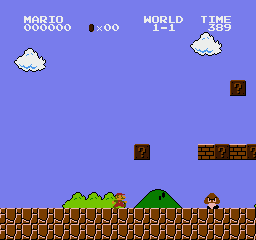
\includegraphics[width=4cm]{img/full_frame.png}\\Obraz generowany przez emulator NES};
				\node[right of=full_frame, xshift=6cm, draw=black] (compressed_frame) {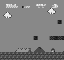
\includegraphics[width=2.5cm]{img/compressed_frame.png} \\Skompresowany obraz};
				\node (model) [right of=compressed_frame, draw = black, minimum height=2cm, xshift=2cm] {Model};
				\node (controller) [right of=model, draw=black, minimum height = 2cm, xshift=1cm, minimum width = 2cm] {Przyciski\\kontrolera\\NES};
				\draw[<-] (compressed_frame.west) -- (full_frame.east) node[midway] {Zmniejszenie\\ rozmiaru i \\ konwersja na skalę \\szarości};
				\draw[<-] (model.west) -- (compressed_frame.east) node[midway]{Konwersja\\na tensor};
				\draw[<-] (controller.west) -- (model.east) node[midway] {Predykcja\\wciśnięć};

			\end{tikzpicture}
		}
	\end{center}
	\caption{Ogólny schemat działania programu}
	\label{fig:sysdiagram}
\end{figure}
\subsection{Emulator NES}

Środowisko gry zostało zaimplementowane przy użyciu emulatora NES opartego na bibliotece \texttt{cynes} \cite{CYNES}. Emulator ten umożliwia dokładną symulację działania konsoli Nintendo Entertainment System, oferując dostęp do pamięci RAM oraz renderowanie obrazu w czasie rzeczywistym.

Emulator działa w dwóch trybach:
\begin{itemize}
	\item \textbf{Tryb okienkowy (windowed)} – pozwala na wizualizację gry oraz interakcję za pomocą klawiatury, co jest przydatne podczas prezentacji działania modeli.
	\item \textbf{Tryb bez okna (headless)} – zoptymalizowany pod kątem wydajności, idealny do procesów trenowania modeli uczenia maszynowego.
\end{itemize}

\subsection{Agent}

Agent w systemie to model decyzyjny, który podejmuje akcje w środowisku gry na podstawie bieżącego stanu. Model ten jest trenowany za pomocą algorytmu Double Q-Learning. Agent:

\begin{itemize}
	\item \textbf{Wejście:} Otrzymuje przetworzony obraz, generowany przez emulator \texttt{cynes}.
	\item \textbf{Wyjście:} Generuje sześć wartości odpowiadających naciśniętym klawiszom:
	      \begin{itemize}
		      \item cztery kierunki ruchu (lewo, prawo, góra, dół),
		      \item dwa przyciski akcji (A i B).
	      \end{itemize}
	\item \textbf{Cel:} Nauka optymalnej strategii, która maksymalizuje sumę nagród za pomocą algorytmu Double Q-Learning.
\end{itemize}

\section{Środowisko gry}

Środowisko składające się wyłącznie z jednego poziomu gry, bez włączonych efektów dźwiękowych.

W danym poziomie gracz/agent ma ograniczony zestaw działań, które mogą być podejmowane w odpowiedzi na bieżący stan gry:
\begin{itemize}
	\item Poruszanie się w poziomie:
	      \begin{itemize}
		      \item Ruch w prawo – pozwala na kontynuowanie gry w kierunku celu.
		      \item Ruch w lewo – ograniczony ze względu na jednokierunkowy projekt poziomu, ale w niektórych sytuacjach może być używany.
	      \end{itemize}
	\item Skakanie:
	      \begin{itemize}
		      \item Gracz/agent może skakać, aby unikać przeszkód, pokonywać przeciwników lub poruszać się między różnymi platformami.
	      \end{itemize}
	\item Stanie w miejscu – brak akcji, co jest domyślnym stanem w przypadku braku aktywności ze strony agenta.
	\item Interakcje z otoczeniem:
	      \begin{itemize}
		      \item Eliminowanie przeciwników poprzez skakanie na nich.
		      \item Zbieranie punktów poprzez interakcje z obiektami (np. monety).
	      \end{itemize}
\end{itemize}

Nie ma możliwości wpływania na inne aspekty gry, takie jak przełączanie poziomów czy modyfikacja otoczenia. Gra kończy się w przypadku ukończenia poziomu, utraty życia lub upłynięcia limitu czasu.
\subsection{Agregacja danych}

Mechanizm agregacji danych zajmuje się odczytem istotnych informacji ze stanu pamięci emulatora, takich jak pozycja Mario, prędkość, aktualny poziom, liczba punktów, a także stan przeciwników. Dane te są później używane do trenowania agenta. Tabela~\ref{tab:nes_memory} przedstawia najważniejsze zmienne i ich adresy w pamięci RAM.

\begin{table}[!ht]
	\centering
	\caption{Zmienne odczytywane z pamięci emulatora NES}
	\label{tab:nes_memory}
	\begin{tabular}{|c|c|p{5cm}|}
		\hline
		\textbf{Adres w RAM}               & \textbf{Nazwa zmiennej} & \textbf{Opis}                                         \\ \hline
		\texttt{0x75A}                     & \texttt{lives}          & Liczba żyć Mario.                                     \\ \hline
		\texttt{0x006D} i \texttt{0x0086}  & \texttt{x}              & Pozycja Mario.                                        \\ \hline
		\texttt{0x0057}                    & \texttt{speed}          & Prędkość pozioma Mario (w postaci liczby ze znakiem). \\ \hline
		\texttt{0x00CE}                    & \texttt{y}              & Pionowa pozycja Mario na ekranie.                     \\ \hline
		\texttt{0x0760}                    & \texttt{level}          & Aktualny numer poziomu gry.                           \\ \hline
		\texttt{0x07DD} do \texttt{0x07E2} & \texttt{score\_bcd}     & Wynik punktowy w formacie BCD (Binary-Coded Decimal). \\ \hline
	\end{tabular}
\end{table}
\section{Realizacja uczenia maszynowego}

Program uczący działa w sposób iteracyjny, realizując kolejne kroki interakcji agenta ze środowiskiem, aktualizując wartości funkcji \(Q_1\) i \(Q_2\), oraz zbierając dane treningowe. Poniżej przedstawiono szczegółowy opis procesu.

\subsection{Pętla gry}
Proces działania programu można podzielić na następujące kroki:
\begin{enumerate}
	\item \textbf{Stan gry (\(s_t\)):} Agent odczytuje aktualny stan gry z obrazu emulatora NES.

	\item \textbf{Wybór akcji (\(a_t\)):}
	      \begin{itemize}
		      \item Zgodnie ze strategią \(\epsilon\)-greedy agent wybiera akcję:
		            \begin{itemize}
			            \item Z prawdopodobieństwem \((1 - \epsilon)\): wybierana jest akcja oparta na predykcji modelu online.
			            \item Z prawdopodobieństwem \(\epsilon\): wybierana jest losowa akcja z zakresu \( \{0, 1, 2, \dots, 6\} \), odpowiadająca kombinacjom klawiszy NES.
		            \end{itemize}
		      \item Akcja jest następnie przekazywana do emulatora jako wejście kontrolera gry.
	      \end{itemize}

	\item \textbf{Następny stan gry (\(s_{t+1}\)):} Emulator NES, po wykonaniu akcji \(a_t\), aktualizuje stan gry i zwraca nowy stan \(s_{t+1}\) oraz nagrodę \(r_t\). Nagroda odzwierciedla skuteczność podjętej akcji w kontekście realizacji celu (np. zwiększenie punktów, przejście poziomu, unikanie przeszkód).

	\item \textbf{Replay Buffer:} Dane z bieżącego kroku (\(s_t, a_t, r_t, s_{t+1}\)) są zapisywane w buforze odtworzeń (ang. Replay Buffer). Jeśli rozmiar bufora przekracza określony próg, najstarsze dane są usuwane, aby zachować ograniczoną wielkość bufora.

	\item \textbf{Trenowanie modelu:}
	      \begin{itemize}
		      \item Gdy bufor odtworzeń osiągnie wystarczającą liczbę próbek, uruchamiany jest proces treningowy.
		      \item Próbki są losowo wybierane z bufora, co zmniejsza korelację między danymi i stabilizuje proces uczenia.
		      \item Na podstawie wybranych próbek aktualizowane są wartości \(Q_1\) i \(Q_2\) zgodnie z algorytmem Double Q-Learning.
	      \end{itemize}

	\item \textbf{Agregacja danych:} Po każdym kroku dane dotyczące gry, takie jak pozycja Mario, wynik, liczba żyć, oraz nagroda, są zapisywane w celu analizy wyników i ewaluacji modelu.
\end{enumerate}

\subsection{Funkcja nagrody \(r\)}

Funkcja nagrody w systemie została zaprojektowana tak, aby odzwierciedlać różne aspekty rozgrywki w grze \textit{Super Mario Bros}. Jej celem jest dostarczenie agentowi sygnałów wspierających naukę skutecznych strategii przechodzenia poziomów. Poniżej przedstawiono kluczowe składniki funkcji nagrody w formie tabeli~\ref{tab:reward_function}.
\begin{table}[!ht]
	\centering
	\caption{Składniki funkcji nagrody}
	\label{tab:reward_function}
	\begin{tabular}{|c|p{7.8cm}|c|}
		\hline
		\textbf{Rodzaj nagrody/kary}                                                        & \makecell{\textbf{Opis}} & \textbf{Zakres} \\ \hline
		\makecell{Nagroda za                                                                                                             \\ postęp w poziomie} &
		\makecell{Nagroda obliczana na                                                                                                   \\ podstawie pozycji poziomej                                                              \\
		\(\text{r}_{pos} = \frac{1}{3220} x_{\text{pos}} - \frac{2}{161}\)}                 &
		\([0,1]\)                                                                                                                        \\ \hline
		\makecell{Nagroda za                                                                                                             \\  zdobycie punktów} &
		\makecell{Nagroda oparta na                                                                                                      \\ zmianie liczby punktów                                                                    \\
		\(\text{r}_{score} = \frac{\Delta \text{score}}{100} \cdot \texttt{score\_delta}\)} &
		\([0, 0.02]\)                                                                                                                    \\ \hline
		\makecell{Nagroda za                                                                                                             \\ ukończenie poziomu} &
		\makecell{Jednorazowa nagroda przyznawana                                                                                        \\ po ukończeniu poziomu.} &
		\([0, 10]\)                                                                                                                      \\ \hline
		\makecell{Kara za śmierć}                                                           &
		\makecell{Kara przyznawana za utratę życia.}                                        &
		\([-10, 0]\)                                                                                                                     \\ \hline
		\makecell{Nagroda za                                                                                                             \\eliminację przeciwników} &
		\makecell{Nagroda przyznawana                                                                                                    \\ za skakanie na wrogów.} &
		\([0,2]\)                                                                                                                        \\ \hline
	\end{tabular}
\end{table}

Łączna nagroda \(r\) jest sumą wszystkich składników nagrody.
\paragraph{Normalizacja funkcji nagrody:}

Normalizacja funkcji nagrody jest kluczowym elementem zapewniającym stabilność procesu uczenia. W systemach takich jak Double Q-Learning, zbyt małe lub zbyt duże wartości nagród mogą prowadzić do problemów z konwergencją algorytmu. Główne cele normalizacji to:

\begin{itemize}
	\item \textbf{Utrzymanie stabilności wartości \(Q\):} Jeśli wartości nagród są zbyt małe, funkcje \(Q(s, a)\) mogą również zbliżać się do zera, co prowadzi do trudności w odróżnianiu jakości różnych akcji. Z kolei zbyt duże wartości nagród mogą powodować eksplozję wartości \(Q(s, a)\), co zakłóca proces uczenia.
	\item \textbf{Przyspieszenie procesu uczenia:} Normalizacja redukuje różnice skali pomiędzy różnymi składnikami nagrody, dzięki czemu algorytm uczy się efektywniej.
	\item \textbf{Zapobieganie dominacji składników nagrody:} Wartości niektórych składników nagrody mogą być znacznie większe niż innych (np. nagroda za ukończenie poziomu w porównaniu do nagrody za eliminację przeciwnika). Normalizacja pomaga wyrównać wpływ poszczególnych składników.
\end{itemize}

W tym systemie nagroda jest normalizowana w każdym kroku na podstawie średniej (\(\mu\)) i odchylenia standardowego (\(\sigma\)) bieżących nagród:
\[
	r_n = \frac{r - \mu}{\sigma}.
\]
\subsection{Model}

Model używany w systemie jest oparty na konwolucyjnej sieci neuronowej (ang. Convolutional Neural Network, CNN). Sieć składa się z warstw konwolucyjnych, normalizujących oraz w pełni połączonych. Architektura modelu jest przedstawiona na rysunku~\ref{fig:modellayers}.

\paragraph{Parametry i wagi:}
Model zawiera około 4 milionów parametrów, co czyni go wystarczająco złożonym, aby efektywnie reprezentować funkcję wartości \(Q(s, a)\) w złożonym środowisku gry. Parametry te obejmują wagi i biasy w warstwach konwolucyjnych oraz w pełni połączonych.

Wagi modelu są inicjalizowane metodą He\cite{he2015} (ang. Kaiming Initialization), co wspiera efektywne uczenie w głębokich sieciach neuronowych. Ta metoda losowo ustawia wartości wag w sposób, który minimalizuje ryzyko eksplozji lub zaniku gradientów w trakcie propagacji wstecznej.

\paragraph{Wygaszanie wag:}
Model implementuje technikę wygaszania wag\cite{krogh1992} (ang. Weight Decay), która jest formą regulacji. Wygaszanie wag zmniejsza wartości parametrów sieci w trakcie procesu uczenia, co zapobiega nadmiernemu dopasowaniu (ang. overfitting). Mechanizm ten działa poprzez dodanie do funkcji kosztu regularizatora w postaci normy L2 wag:
\[
	L = L_{\text{loss}} + \lambda \|W\|_2^2,
\]
gdzie \(L_{\text{loss}}\) to główna funkcja kosztu, \(W\) to wektor wag modelu, a \(\lambda\) to współczynnik regularyzacji.
\begin{figure}[!ht]
	\begin{center}
		\begin{tikzpicture}[node distance=1.0cm]
			\node[draw, rectangle, minimum width=4cm, minimum height=0.7cm] (input) {Wejście: [60x64]};
			\node[draw, rectangle, minimum width=4cm, minimum height=0.7cm, below of=input] (conv1) {Warstwa konwolucyjna: 1 $\rightarrow$ 32};
			\node[draw, rectangle, minimum width=4cm, minimum height=0.7cm, below of=conv1] (bn1) {Warstwa normalizująca: 64 kanały};
			\node[draw, rectangle, minimum width=4cm, minimum height=0.7cm, below of=bn1] (conv2) {Warstwa konwolucyjna: 32 $\rightarrow$ 64};
			\node[draw, rectangle, minimum width=4cm, minimum height=0.7cm, below of=conv2] (bn2) {Warstwa normalizująca: 64 kanały};
			\node[draw, rectangle, minimum width=4cm, minimum height=0.7cm, below of=bn2] (flatten) {Spłaszczenie: 1x30720};
			\node[draw, rectangle, minimum width=4cm, minimum height=0.7cm, below of=flatten] (fc1) {Warstwa gęsta: 30720 $\rightarrow$ 128};
			\node[draw, rectangle, minimum width=4cm, minimum height=0.7cm, below of=fc1] (fc2) {Warstwa gęsta: 128 $\rightarrow$ 6};
			\node[draw, rectangle, minimum width=4cm, minimum height=0.7cm, below of=fc2] (output) {Wyjście: 6 wartości};

			% Connections
			\draw[->] (input) -- (conv1);
			\draw[->] (conv1) -- (bn1);
			\draw[->] (bn1) -- (conv2);
			\draw[->] (conv2) -- (bn2);
			\draw[->] (bn2) -- (flatten);
			\draw[->] (flatten) -- (fc1);
			\draw[->] (fc1) -- (fc2);
			\draw[->] (fc2) -- (output);

		\end{tikzpicture}
	\end{center}
	\caption{Warstwy modelu}
	\label{fig:modellayers}
\end{figure}

